\documentclass{article}

\PassOptionsToPackage{numbers,compress}{natbib}
 \usepackage{neurips_2025}
\usepackage[utf8]{inputenc} % allow utf-8 input
\usepackage[T1]{fontenc}    % use 8-bit T1 fonts
\usepackage{hyperref}       % hyperlinks
\usepackage{url}            % simple URL typesetting
\usepackage{booktabs}       % professional-quality tables
\usepackage{amsfonts}       % blackboard math symbols
\usepackage{nicefrac}       % compact symbols for 1/2, etc.
\usepackage{microtype}      % microtypography
\usepackage{xcolor}         % colors
\usepackage{amsmath}
\usepackage{amssymb}
\usepackage[]{tikz}
\usepackage{graphicx}
\usepackage{subcaption}

\usetikzlibrary{positioning}
\title{Hidden Market Regimes in Equity Returns via Hidden Markov Models}


\author{Charlie Kushelevsky, Parth Paliwal, Max Zhang, Cole Carter}

\begin{document}

  \vspace{-0.4in}
\maketitle

\begin{center}
    \href{https://github.com/charliekush/latent-market-regimes-hmm}{https://github.com/charliekush/latent-market-regimes-hmm}
\end{center}

\subsection*{Problem Description}

Financial markets appear noisy from day to day, yet empirical evidence suggests that price movements are driven by a small number of persistent latent ``regimes,'' such as low-volatility growth periods, high-volatility downturns, or transitional sideways phases (e.g.\ bull trends, bear markets, high volatility). These regimes are not directly observable, but they affect return distributions, volatility clustering, and risk. 

The goal of this project is to use a Hidden Markov Model (HMM) to uncover latent market regimes from historical equity return data. We treat the daily market return as the observed variable and the underlying regime as a hidden state that evolves slowly over time. Using probabilistic reasoning, expectation maximization (Baum-Welch), and sequence inference (Viterbi), we want to characterize how many regimes best describe the behavior of the market and how persistent these regimes are. This problem uses the course topics of latent variable modeling, EM-based learning, and probabilistic inference.


We seek to answer questions such as: (1) How many distinct regimes best capture the distributional structure of daily market returns? (2) What statistical properties (mean, variance) define each regime?  (3) How persistent are different regimes, and how frequently do transitions occur?  (4) Do inferred high-volatility states align with known market stress periods, such as the 2008 crisis or the 2020 COVID crash?

\subsection*{Dataset}
We will use daily adjusted closing prices of the SPDR S\&P~500 ETF (ticker: SPY), obtained from publicly available historical data through the \texttt{yfinance} Python API. The dataset will span  1958 through 2025, covering multiple market cycles including the dot com aftermath, the 2008 global financial crisis, the long 2010-2019 expansion, the COVID crash, and the 2022-2023 inflationary period.


Preprocessing consists of: (1) restricting the dataset to valid trading days; (2) computing daily log returns,
\[
r_t = \log\!\left(\frac{P_t}{P_{t-1}}\right),
\]
where $P_t$ is the adjusted closing price; (3) dropping missing values from holidays and non-trading days; and (4) optionally standardizing returns for numerical stability. No additional feature engineering is required for the baseline HMM.

This dataset is well suited for sequence models because it provides a long, continuous, high quality return time series, enabling reliable estimation of persistent hidden dynamics.

Our dataset of daily SPY log returns are naturally sequential and are well-suited to HMM for two properties (regime-like behavior and volatility clustering). The hidden state \(S_t\) represents a small number of regimes and the transition matrix specifies how likely the market is to move to another regime or remain the same. The regimes cannot be directly observed and instead, we only see noisy return from them.

But the data do not perfectly satisfy the HMM assumptions.The data-generation process is influenced not just by short term volatility but also long-run macroeconomic forces, structural breaks, and investor behavior that are not fully captured by a small number of discrete regimes. Therefore we treat the HMM as a simplified approximation so our data fits the markov property \(P(S_t | S_{1,..,t-1}) = P(S_t|S_{t-1}))\) meaning that the current regime state only depends on the previous regime. This is a reasonable assumption because market conditions and volatility are locally persistent, meaning that a high volatility crisis day is less likely to be followed by a low volatility calm regime.



Our dataset is well-suited to HMMs since it looks like there is a hidden model that generates a sequence over a period of time. The dataset takes a series of log returns; however, there are series of different states that the market undergoes that can be summed up to stable, volatile, or normal periods of time. These cannot be observed directly, but instead, they affect the returns, and these different states are the hidden states within an HMM. 
Furthermore, we can utilize Gaussian emissions when looking at a specific hidden state and a known solution. We know that at each hidden state, there are different emission variances and means that can be observed in the \texttt{gauss\_hmm} python file. 

Although our dataset is not a perfect fit for the HMM, it is more than well-suited to be an HMM, particularly the Gaussian HMM with emphasis on the Markov property, which allows for quick, easy, and accurate predictions.


\subsection*{Methodology}

We will model the return sequence $\{r_t\}$ using a $K$-state Hidden Markov Model with Gaussian emissions. Each hidden state $S_t \in \{1,\dots,K\}$ represents an unobserved market regime, while the emission distribution $r_t \mid S_t = k \sim \mathcal{N}(\mu_k, \sigma_k^2)$ captures the characteristic return behavior of that regime. The transition matrix encodes the persistence and switching behavior between regimes, which we expect to be highly skewed toward self-transitions.

Model parameters (initial state distribution, transition probabilities, and emission parameters) will be learned with the Baum-Welch algorithm (EM). We will experiment with different values of $K$ (e.g., $K=2,3,4$) to compare fit, interpretability, and stability. After learning, we will apply the Viterbi algorithm to infer the most likely regime sequence over time and examine whether high-volatility regimes correspond to known historical events.

Evaluation will include log-likelihood, qualitative inspection of decoded regimes, and analysis of transition probabilities and expected regime durations. If time permits, we may extend the model to incorporate additional observable variables such as realized volatility or trading volume.
\subsection*{Background}
Our project utilizes the Bayesian network with continuous variables. In class, we learned discrete Bayesian network (eg. Regime \(\in\) {bull, bear, crash}) where every variable takes values in a finite set and each node is associated with a CPT. If we modeled both regimes and returns as discrete, we would have:

\begin{itemize}
\item hidden state: \(S_t \in \{1,\dots,K\}\)
\item discretized return: \(\tilde r_t \in \{\text{“big loss”}, \text{“small loss”}, \text{“flat”}, \text{“small gain”}, \text{“big gain”}\}\) and the emission model would be a CPT \(P(r_t = x \mid S_t = k)\)
\item With continuous Bayesian network, our variables take real values (eg. return\_t \(\in  \mathbb{R}\), Volatility\_t  \(\in  \mathbb{R}\))
\item hidden state \(S_t \in \{1,\dots,K\}\) is still discrete,
\item observed return \(r_t \in \mathbb{R}\) is continuous
\item hidden state \(S_t \in \{1,\dots,K\}\) is still discrete,
\item and the local conditional for the emission node is Gaussian:
\[r_t \mid S_t = k \sim \mathcal{N}(\mu_k,\sigma_k^2)\].
\item Instead of a CPT for \(P(r_t \mid S_t)\), we have a parametric density with regime-specific parameters \((\mu_k,\sigma_k^2)\).
\[
p(r_t \mid S_t)=\prod_{k=1}^K \mathcal{N}(r_t \mid \mu_k,\sigma_k^2)^{\mathbf{1}[S_t = k]}
\]




\end{itemize}
\subsection*{Inference}
The hidden chain \(S_{1:T}\) is still discrete, so forward-backward and Viterbi operate using sums over regimes (no integrals over continuous hidden variables).

The only continuous part is evaluating the likelihood term
\[
p(r_t \mid S_t = k) = \mathcal{N}(r_t \mid \mu_k,\sigma_k^2),
\]
instead of looking up a CPT entry \(P(\tilde r_t \mid S_t)\).

\subsection*{Learning}

In a fully discrete BN, the M-step would update CPT entries via normalized counts.
In our continuous BN, the M-step for emissions updates \(\mu_k,\sigma_k^2\) via weighted Gaussian fitting:
\[
\mu^k= \frac{\sum_t \gamma_t(k)\, r_t}{\sum_t \gamma_t(k)}, \qquad \hat{\sigma}_k^2 = \frac{\sum_t \gamma_t(k)\,\big(r_t - \hat{\mu}_k\big)^2}{\sum_t \gamma_t(k)},
\]
 where \(\gamma_t(k)=P(S_t=k\mid r_{1:T})\) are the soft assignments from the E-step.
For our EM algorithm, we use a specialized instance of EM called the Baum-Welch algorithm. This algorithm takes a generalized EM and applies it to a HMM. A generic EM algorithm would require summing over all possible hidden states sequences which is inefficient. The Baum-Welch algorithm is much more efficient as it uses the forward backwards algorithm to compute the required expectations in \(O(TK^2)\) time instead of exponential time. We train the model for up to 100 EM iterations, using a convergence tolerance of \(10^{-4}\) based on the change in log-likelihood between iterations. In practice, the algorithm typically converged within 20-40 iterations depending on the number of regimes. To ensure numerical stability, especially for long financial sequences, we applied log-domain computations in the forward-backward pass and introduced small smoothing constants in the M-step to prevent zero probabilities.

\begin{itemize}
\item Initialize \(\pi, A, \mu_k, \sigma_k^2\) (e.g., random, k-means on returns, or simple guesses).
\item E-step (forward-backward): Use current parameters to compute \(\gamma_t(k)\) and \(\xi_t(i,j)\) from the returns series. This gives a soft segmentation of history into regimes.
\item M-step: Update \(\pi, A\) from \(\gamma, \xi\) (discrete BN part). Update \(\mu_k, \sigma_k^2\) using the weighted formulas above (continuous BN part). Only difference is the M-step where we update using weighted formulas instead of what we learned in class.
\item Repeat until log-likelihood stops improving.
\end{itemize}

\subsection*{Implementation}
For the analysis of the transition probabilities, we have to examine how the regimes stay at a certain stage for a period of time, and we can compare which regimes with the longest durations and the regimes with the shortest durations that fluctuate much more often. We also need to take into account the entries that are “off diagonal”, which gives the user a visualization of regime switches. This tells a story of whether the market is trending downwards gradually or experiencing a very volatile fluctuation. We also want to find a reasonable duration for the regime. We want to find the average length of a single regime, and observe that certain regimes of lower fluctuations have longer periods of time of slow regression. But at times of fast degradation, it should be a very quick period of time. 

Next, the benchmark that we chose was the single regime Gaussian model. Furthermore, we also used historical data as a benchmark to mark regimes of short duration but very high volatility. We can see that during times of historical financial complications, it should correspond to the timing of high volatility. We should expect to see a correlation between higher stress on the model's regimes during periods of market stress. This can be seen as a qualitative way to record evidence of the structure of data. 

The qualities that we should analyze when inspecting decoded regimes are the differences in states between each regime. Double-checking the timing of each of the regimes and seeing if they match up with periods of crisis, and if there are long periods of slight or normal growth instead of longer periods of volatility. Checking the length of the models and observing that it should reflect a calm and steady state instead of a short and volatile state over a longer period of time. Lastly, it should be a proper interpretation of the economy and see that the Gaussian HMM is capturing data that is readable and useful. 


To train the test split based on the time span, as we are using the early parts of the dataset as training and the latter as a test. Thus, this means that we are going to train the test based on the split by time. This means that depending on the data from the past, we can evaluate the data in the future from the trainings. Furthermore, for each value of K, the hidden states, we can fit an HMM for the training. 

We train the log-likelihood and its AIC and BIC, which will give us a reading of the fit and how the model will perform. Furthermore, it also allows us to identify the complexity of the model. A lower AIC BIC value indicates that there is a tradeoff between how the model performs and the number of parameters. We can use these values to compare the models with varying K values. We will find HMMs and compare them based on different values of K by finding the AIC BIC values to prevent overfitting and testing the log-likelihood to assess the predictions of the models. 

\section*{Modeling and Inference}

To formalize the market regime detection problem, we use a probabilistic generative model that
maps the observed return sequence to a sequence of latent regimes. We adopt a $K$-state Hidden
Markov Model (HMM) that encodes specific assumptions about how regimes evolve over time and
how they generate daily returns. In this section we describe the assumptions, parameters, and
dependency structure of this model, and explain how they relate to financial intuition.

\subsubsection*{Assumptions}

Our HMM relies on several standard but important structural assumptions.

\paragraph{First-order Markov dynamics.}
We assume the hidden regimes follow a first-order Markov chain:
\[
P(S_t \mid S_{1:t-1}) = P(S_t \mid S_{t-1}).
\]
This captures the idea that market conditions are locally persistent. Volatility and risk tend to
evolve gradually, so today's regime is well summarized by yesterday's regime rather than the full
history.

\paragraph{Conditional independence of returns given the regime.}
Each daily log return $r_t$ is conditionally independent of past returns once the current regime
is known:
\[
P(r_t \mid S_{1:t}, r_{1:t-1}) = P(r_t \mid S_t).
\]
Intuitively, the regime already encodes the relevant information about volatility and drift. Once
we know which state the market is in, additional past returns do not change the distribution of
$r_t$.

\paragraph{Gaussian emission model.}
Within each regime $k$ we model returns as Gaussian:
\[
r_t \mid S_t = k \sim \mathcal{N}(\mu_k, \sigma_k^2),
\]
where $\mu_k$ is the mean daily return and $\sigma_k^2$ is the variance. This reflects the
empirical observation that, conditional on a volatility regime, daily returns are approximately
Gaussian even though the unconditional distribution is heavy-tailed.

\paragraph{Piecewise stationarity and chronological training.}
We assume that the emission parameters $(\mu_k, \sigma_k^2)$ are constant over time within a
regime, so the process is piecewise stationary: the distribution of returns is stable as long as the
market remains in the same state. At the same time, we never shuffle dates. We train on the
earlier portion of the sample and evaluate on later years, mimicking a realistic forecasting
setting and avoiding information leakage from the future into the past.

\subsubsection*{Parameters and financial interpretation}

Let $K$ denote the number of regimes. The HMM is parameterized by:

\medskip
\noindent
\textbf{Initial state distribution.}
The probability that the market starts in regime $k$ is
\[
\pi_k = P(S_1 = k), \qquad k = 1, \dots, K.
\]

\medskip
\noindent
\textbf{Transition matrix.}
The dynamics of regime switches are governed by a $K \times K$ transition matrix
\[
A_{ij} = P(S_{t+1} = j \mid S_t = i).
\]
Diagonal entries $A_{kk}$ encode persistence of regime $k$, while off-diagonal entries capture
switches between regimes. The expected duration of regime $k$ under this Markov chain is
\[
\mathbb{E}[D_k] = \frac{1}{1 - A_{kk}},
\]
so large diagonal probabilities correspond to long-lived regimes.

\medskip
\noindent
\textbf{Emission parameters.}
Each regime $k$ has a mean return $\mu_k$ and variance $\sigma_k^2$. Financially, these
parameters distinguish different market environments:

\begin{itemize}
    \item high-volatility regimes have large $\sigma_k$;
    \item bull-market regimes have positive $\mu_k$;
    \item crisis regimes may combine negative $\mu_k$ with elevated $\sigma_k$.
\end{itemize}

Together, $(\pi, A, \{\mu_k, \sigma_k^2\}_{k=1}^K)$ define the complete generative story for the
return sequence under the HMM.

\subsubsection*{Structure of dependencies}

Figure~\ref{fig:hmm-structure} summarizes the dependency structure of our model. The hidden
regimes $(S_1, \dots, S_T)$ form a Markov chain along the horizontal axis, and each daily log
return $X_t$ is generated conditionally on the corresponding hidden regime $S_t$:

\[
S_1 \rightarrow S_2 \rightarrow S_3 \rightarrow \cdots \rightarrow S_T
\]
\[
\downarrow \qquad \downarrow \qquad \downarrow \qquad \qquad \downarrow
\]
\[
X_1 \quad\;\; X_2 \quad\;\; X_3 \quad\;\; \cdots \quad\;\; X_T.
\]

Horizontal arrows encode the temporal evolution of regimes, while vertical arrows represent the
emission of observable returns from each regime. This structure matches the intuition that
market states evolve slowly over time and that each day's return is a noisy reflection of the
current underlying regime.

\begin{figure}[h]
\centering
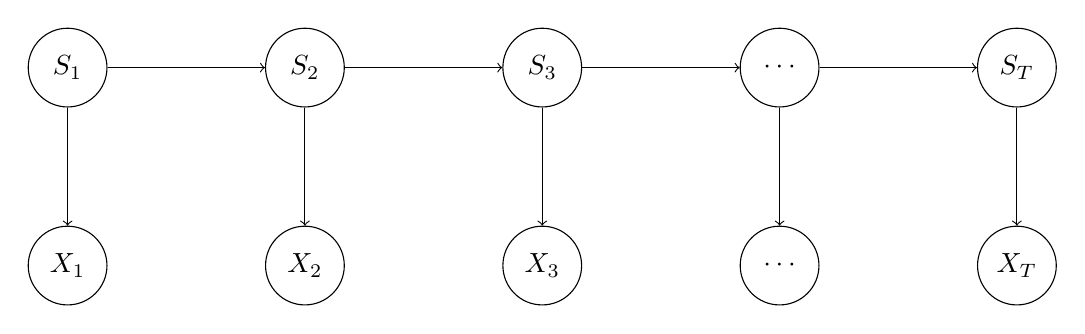
\begin{tikzpicture}[
    node distance = 2.0cm,
    hid/.style = {circle, draw, minimum size=1cm},
    obs/.style = {circle, draw, minimum size=1cm}
]

\node[hid] (S1) {\(S_1\)};
\node[hid, right=of S1] (S2) {\(S_2\)};
\node[hid, right=of S2] (S3) {\(S_3\)};
\node[hid, right=of S3] (Sdots) {\(\cdots\)};
\node[hid, right=of Sdots] (ST) {\(S_T\)};

\node[obs, below=1.5cm of S1] (X1) {\(X_1\)};
\node[obs, below=1.5cm of S2] (X2) {\(X_2\)};
\node[obs, below=1.5cm of S3] (X3) {\(X_3\)};
\node[obs, below=1.5cm of Sdots] (Xdots) {\(\cdots\)};
\node[obs, below=1.5cm of ST] (XT) {\(X_T\)};

\draw[->] (S1) -- (S2);
\draw[->] (S2) -- (S3);
\draw[->] (S3) -- (Sdots);
\draw[->] (Sdots) -- (ST);

\draw[->] (S1) -- (X1);
\draw[->] (S2) -- (X2);
\draw[->] (S3) -- (X3);
\draw[->] (Sdots) -- (Xdots);
\draw[->] (ST) -- (XT);

\end{tikzpicture}
\caption{HMM structure: hidden regimes \(S_t\) and observed log returns \(X_t\).}
\label{fig:hmm-structure}
\end{figure}

\begin{itemize}
    \item Horizontal arrows: Markov transitions between regimes.
    \item Vertical arrows: each regime \(S_t\) generates an observation \(X_t\).
\end{itemize}
\subsection*{Evaluation Criteria}
To compare HMMs with different numbers of regimes, we evaluate each model using both the training and heldout test set log likelihood. Because financial data is time dependent, we apply a chronological train test split, training on early data and evaluating later ones to avoid information leakage. This allows us to measure predictive accuracy and reduces the risk of overfitting historical data.

We also incorporate the Akaike Information Criteria (AIC) and Bayesian Information Criterion (BIC) to compare models with different values of \(K\). Both AIC and BIC penalize model complexity by adding a term proportional to the number of parameters allowing us to quantify the tradeoff between goodness of fit and simplicity. Lower values of \(K\) indicate a more conservative model.  Thus, our selection of \(K\) is based jointly on test log likelihood and information criteria, ensuring the chosen model generalizes well and avoids unnecessary complexity. 

\section*{Results and Discussion}

\subsection*{Exploring Multiple Model Configurations}

We trained the HMMs with K = 2,3,4 latent regimes to compare models more easily. Increasing K expands the capacity of the model by allowing a more enhanced mixture of Gaussian components. As expected, the in-sample log-likelihood strictly increased with larger K as shown in the table above. Both AIC and BIC become more negative as K increases, indicating that the improvement in likelihood outweighs the penalty for additional parameters. According to BIC, the favored model is K = 4.

\begin{table}[h!]
\centering
\caption{Model comparison for different values of \(K\).}
\label{tab:model-comp}
\begin{tabular}{c c c c c}
\hline
\(K\) & Train LL & Test LL & AIC & BIC \\ \hline
2 & 34914.6 & 22112.9 & \(-69{,}815.2\) & \(-69{,}764.7\) \\
3 & 35056.8 & 21851.5 & \(-70{,}085.7\) & \(-69{,}984.6\) \\
4 & 35307.0 & 22347.6 & \(-70{,}568.0\) & \(-70{,}402.0\) \\ \hline
\end{tabular}
\end{table}

\subsection*{Quantitative Properties of the Learned Regimes}

The emission parameters of the K=4 model reveal a mixture of one degenerate state and three economically interpretable regimes. Each regime k is characterized by a Gaussian emission density.

\begin{table}[h!]
\centering
\caption{Emission parameters of the \(K=4\) HMM.}
\label{tab:emission-params}
\begin{tabular}{c c c}
\hline
Regime & Mean & Std \\ \hline
0 & \(-0.228997\) & \(\approx 0\) (degenerate) \\
1 & \(-0.000909\) & \(0.019021\) \\
2 & \(0.000744\) & \(0.004539\) \\
3 & \(0.000453\) & \(0.008073\) \\ \hline
\end{tabular}
\end{table}

This reflects a limitation of Gaussian HMMs, which cannot accommodate heavy tails. Instead, the model allocates an entire regime to an extreme crash day. The remaining three regimes form a coherent structure. Regime 1 exhibits high volatility and slightly negative mean returns, representing crisis conditions. Regime 2 is characterized by very low volatility and positive mean returns, corresponding to calm bull markets. Regime 3 displays moderate volatility and slightly positive returns, forming the background state that dominates ordinary trading. As shown in Figure~\ref{fig:return-distribution}, Regime 1 has the widest return distribution, consistent with the high-volatility stress periods.

\subsection*{Qualitative Interpretation and Model Behavior}

Regime 2 corresponds to long bull market phases defined by stable price appreciation and low realized volatility. Regime 3 appears during typical trading environments, marked by moderate yet persistent fluctuations about a gradually increasing trend. Regime 1 coincides with high-volatility stress periods; because its mean return is slightly negative and its standard deviation almost four times that of Regime 2, it accurately captures crisis dynamics. As shown in Figure~\ref{fig:price-regimes}, the price series is segmented into distinct regimes that align with major market events, and Figure~\ref{fig:regime-sequence} highlights long stretches of calm periods punctuated by crisis spikes.

\begin{figure}[ht]
\centering
\includegraphics[width=\textwidth]{../plots/regimes.pdf}
\caption{Price series colored by inferred regimes.}
\label{fig:price-regimes}
\end{figure}

\begin{figure}[ht]
\centering
\includegraphics[width=\textwidth]{../plots/sequence.pdf}
\caption{Decoded regime sequence over time.}
\label{fig:regime-sequence}
\end{figure}

\begin{figure}[ht]
\centering
\includegraphics[width=0.9\textwidth]{../plots/return_hist.pdf}
\caption{Return distributions by regime.}
\label{fig:return-distribution}
\end{figure}

\begin{figure}[ht]
\centering
\includegraphics[width=0.85\textwidth]{../plots/convergence.pdf}
\caption{Log-Likelihood vs. EM Iteration.}
\label{fig:em-convergence}
\end{figure}

\subsection*{Convergence, Stability, and Scalability}

The EM algorithm converged smoothly for every value of K. The log-likelihood increased monotonically at each iteration, and scaled forward-backward recursions prevented numerical underflow. No irregularities in parameter updates were observed aside from the expected behavior of the singleton crash state in the K=4 model. Each iteration of EM requires \(O(K^2 T)\) operations, and Figure~\ref{fig:em-convergence} shows the stable ascent of the training objective.


\section*{Conclusion}
In conclusion, our analysis shows that a four-state Hidden Markov Model provides the strongest evidence of underlying structure in daily S\&P~500 returns. As the number of regimes increases, the in-sample likelihood improves consistently, and both AIC and BIC become more negative. These trends point towards the fact that the added parameters contribute real value instead of simply overfitting. The model selection criteria indicate that \(K\)=4 is the best-supported configuration, further suggesting that market behavior is not well captured by only two or three latent regimes.

The emission parameters of the \(K\)=4 model also reveal three economically meaningful regimes and one degenerate crash state. The interpretable regimes correspond to calm bull markets with very low volatility, normal trading conditions with moderate fluctuations, and crisis periods with large negative shocks and elevated variance. The degenerate state highlights the limitation of Gaussian HMMs which is their inability to represent heavy-tailed return distributions. Regardless, the structure of the remaining regimes align closely with established financial intuition regarding volatility clustering and market cycles.

Across all the tested values of \(K\), the EM algorithm converged smoothly, and the forward-backward recursions produced stable updates without issues. The regime sequences behave consistently and correspond well with known patterns in market behavior. Overall, the results demonstrate that HMMs offer a powerful framework for uncovering persistent and interpretable dynamics in financial time series, however future extensions could further improve the model's ability to handle extreme events.

\section*{Contributions \& Learnings}
\textbf{Charlie} \\
I contributed technical components of the project, including data collection and preprocessing, implementing the log-return pipeline, building and debugging the Gaussian HMM, running EM training and model selection, and performing the regime analysis with plots and statistical summaries. I also contributed a lot of the write up and converted groupmates writeup contributions to \LaTeX.

Through this project, I developed a stronger understanding of how probabilistic models behave on real financial time series, especially the practical challenges of EM convergence, numerical stability, and interpreting latent states in an economic context. Working with a full modeling pipeline solidified my intuition about volatility regimes and improved my ability to translate theoretical HMM concepts into a working system.

\textbf{Cole} \\
Something that I learned while working on this project is the power of HMMs and how they can be applied. I think that in class it seemed like it would be useful, but it wasn't until seeing them applied to a real dataset that I fully understood. For instance, being able to tell that the S\&P shows bull signals with low volatility, as it is known to do, is quite impressive.


\textbf{Max} \\
Helped with results analysis\\


\textbf{Parth} \\

One thing that I learned is that HMMs are able to not only predict but also help show how different hidden states can affect the model's output. For example it was able to distinguish normal days from crisis days without. It gave me a better and more practical understanding of how HMMs work and just how useful they can be.


\subsection*{LLM Usage}
Used LLMs to help write up report in \LaTeX as well as some assistance plotting.


\pagebreak


\bibliographystyle{abbrvurl}
\bibliography{references}
\end{document}
